\documentclass[12pt]{article}
\usepackage{common}
\usepackage{hyperref}
\hypersetup{colorlinks,urlcolor=blue}
\setlength{\parindent}{0cm}
\title{General game-playing applied to 2048}
\author{Paul Lisker and Ahmed Ahmed}
\begin{document}
\maketitle{}

\section{Introduction}
General Game Playing (GGP) is a sub-field of Artificial Intelligence that seeks to develop agents that are capable of playing many games rather than being tailored and limited to particular game. GGP has been a popular subject of AI research, particularly over the past decade. The goal of GGP is to create programs that are capable of successfully playing more than one game. As such, a successful GGP agent will not have algorithms tailored to a particular game, but rather generalized algorithms that can be successful when applied to various different games (though occasionally of the same domain---that is, games that are similar in nature). For an illustrative example on the difference between a regular game playing agent and a GGP agent, we can look at IBM's famous Deep Blue computer. This computer ran an AI program that was tailored to the goal of winning a game of chess; however, this program would have been unusable for other games. On the other end of the spectrum, successful GGP programs can play---albeit perhaps less effectively than a dedicated algorithm---more games than just one, or play games that would otherwise be intractable for specialized algorithms.\\

The requirements of General Game Playing, then, necessitate the use of algorithms that are not domain-specific. in other words, it must use algorithms that can operate with a broad spectrum of games without being dependent on shared rules between said games. Among this class of algorithms is Monte Carlo Tree Search (MCTS), a class of algorithms for finding optimal choices in a decision space by taking random sample simulations and building a search tree according to their results. We explore this algorithm with more in Section 2. Among other benefits, MCTS provides an alternative to the traditional approach to combinatorial games---MiniMax algorithms---especially in games of nontrivial size or for those in which no reliable heuristic has been developed, two situations in which MiniMax often fails.\\

In this project, we apply a version of a Monte Carlo Tree Search algorithm to the domain of games surrounding the popular puzzle game \textit{2048}. We also analyze the algorithm's performance, and, in the case of the original \textit{2048} game, compare its effectiveness to published heuristic AI approaches.\\


\section{Background and Related Work}

\subsection{Introduction to 2048}
\href{https://gabrielecirulli.github.io/2048/}{\textit{2048}} is a single-player puzzle game developed by Gabrielle Cirulli that was a viral hit in 2014\cite{twentyfortyeight}. This game consisted of a $4\times4$ grid in which each cell is either empty or contains a tile with a power of two number. In each move, the player chooses a direction in which to slide all the tiles with the goal of having tiles of the same number collide to merge and create a tile of their sum. After each move, a new tile is spawned randomly in any empty cell. The game's goal is to reach the eponymous tile; it continues until (1) there are no more available moves---no more merges possible or open tiles---or (2) the 2048 tile is reached, though at that point the user is given the option to continue beyond to form higher tiles.\\

For this project, we expand the domain of the game \textit{2048} by creating what we refer to as \textit{generalized-2048}. This class of games include modifications to the grid size of the original game and to the scoring policy. As such, though each game is indubitably similar to the original game, each has its own quirk and strategy that requires unique strategies for success.\\


\subsection{Algorithm: Monte Carlo Tree Search}
The Monte Carlo Tree Search is among the most important algorithms in the field of General Game Playing today; its use ``has been widely adopted in GGP research'' \cite{ggp_review}. The main impetus for using MCTS as a principal algorithm in the building of GGP programs is its wide adaptability across games and the proven success in games that, until then, had proven intractable.\\

In 2006, Monte Carlo Tree Search came to prominence after it was successfully used to progress in the building of agents that could play in the game of Go. At the time, AI agents were competitive against humans with small boards, but not yet competitive at standard $19\times19$ boards. However, since then, Google's AlphaGo initiative has created a program successfully integrating deep neural networks with an MCTS approach that, earlier this year, became the first AI winner against a professional, human player \cite{nature_alpha_go, alpha_go}. Despite its clear and proven advantages, however, ``the main disadvantage of MCTS is that it makes very limited use of game-related knowledge, which may be inferred from a game description'' \cite{ggp_review}.\\

MCTS is essentially a class of techniques for traversing  game-trees. Such game trees are an especially convenient model for combinatorial games such as \textit{2048}---that is, sequential, discrete, full-information games. Therefore, this project most directly draws off of the concepts of uninformed and heuristic search that we explored earlier in this course. Additionally, as its name implies, the MCTS algorithm does have a Monte Carlo component: it uses sampling in order to inform its search. This concept of using of sampling methods to find approximate answers to otherwise intractable problems was explored in this course in the context of particle filters in Bayes Nets.\\

Monte Carlo Tree Search algorithms proceed in four main steps: (1) selection, (2) expansion, (3) simulation, and (4) back-propagation. As the algorithm searches the game tree from its current state, it proceeds with each of these four steps in each iteration until some computational limit is reached---typically a certain time limit, or number of iterations---at which point the best discovered move is chosen. A graphical representation of the algorithm can be seen in \textbf{Figure 1}.

\paragraph{Selection} In this first step, the algorithm---beginning at the root node---proceeds along the expanded tree to find a node to expand from the built game tree. This selection typically takes place with the use of some confidence algorithm. A common one---and the one used in our project---is the Upper Confidence Bounds applied for Trees (UCT) algorithm. Ultimately, this results in actions that have been more effective in the past being tested more frequently.

\paragraph{Expansion} With the node selected, the algorithm proceeds to expand the game tree one step with the available moves.

\paragraph{Simulation} From the new node(s) added, the algorithm proceeds to run a random simulation until a termination step is reached.

\paragraph{Back-Propagation} The ultimate score achieved by the simulation is then back-propagated to the nodes visited in the Selection and Expansion steps for use in the decision-making steps of the next iteration of the algorithm.\\

\begin{figure}[h]
\centerline{\fbox{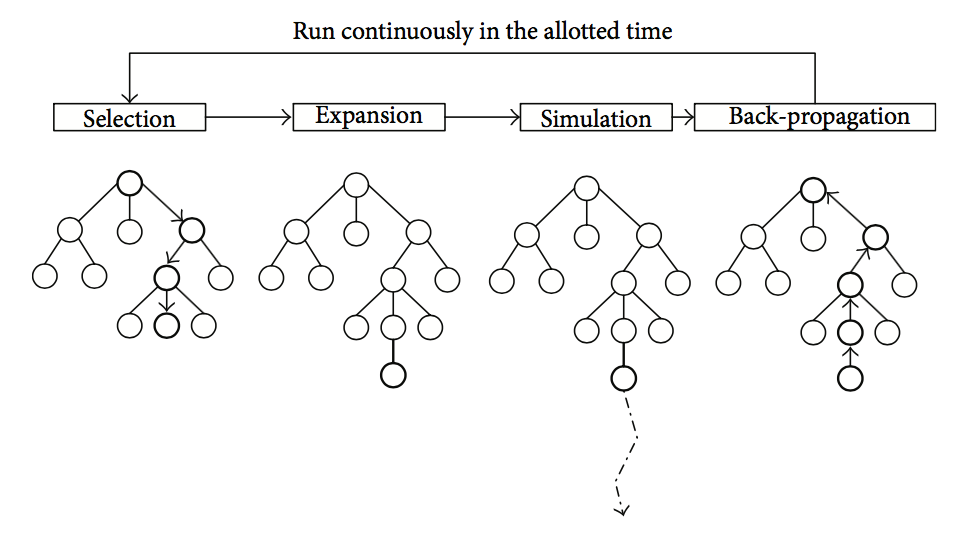
\includegraphics[width=6in]{images/mcts}}}
\caption{The four key steps of the Monte Carlo Tree Search algorithm are represented graphically for a given game tree.}
\end{figure}

\subsection{Published solutions}
Though heuristic search agents have been used to solve \textit{2048} and go beyond the 2048 tile to reach higher tiles and maximize score, to our knowledge this project is the first instance of expanding \textit{2048} to create \textit{generalized-2048} implementations and create general game playing agents to solve them. As such, we briefly discuss heuristic search solutions.\\

As the game went viral a couple of years ago, the AI game-playing community went to work at publishing several automated 2048 players. With this being a single-player game against a computer opponent, the principal approach taken by many implementations has been of leveraging MiniMax \cite{stackoverflow}. However, the most successful implementation of a heuristic search algorithm noted that the random spawning of tiles made this game more suited to an ExpectiMax approach, and it is this version that achieved the impressive 32768 tile. Furthermore, their computationally efficient implementation and accurate heuristics led to impressive success. After running their algorithm one hundred times, the proportion of games in which the following tiles was reached at least once is as follows:
\begin{description}
\item[\textbf{2048:}] 100\%
\item[\textbf{4096:}] 100\%
\item[\textbf{8192:}] 100\%
\item[\textbf{16384:}] 94\%
\item[\textbf{32768:}] 36\%
\end{description}

These impressive statistics were achieved with highly refined heuristics granting bonuses to empty tiles and penalties for non-monotonic rows. Ultimately, the refined heuristics had a dramatic effect: ``the algorithm went from achieving the 16384 tile around 13\% of the time to achieving it over 90\% of the time'' \cite{stackoverflow}. Ultimately, statistics such as these highlight the benefit of a highly-refined algorithm designed for a particular game; truly general game playing agents, by the very definition of the term, cannot benefit from heuristics such as these. After all, ``general game playing expertise depends on intelligence on the part of the game player rather than intelligence of the programmer of the game player'' \cite{ggp_competition}.

\medskip

\section{Problem Specification}
In this project, we aim to build an artificial intelligence program that can play an arbitrary game in the \textit{generalized-2048} class of games. We define \textit{generalized-2048} as the set of games with move and tile-spawning rules equivalent to those of standard \textit{2048}, except that (1) the game may have an arbitrary board size $n \times m$, where, for practicality, $n, m \in \{3,4,5\} $ and (2) the game may have an arbitrary score function $R$, instead of the standard cumulative score of merged tile values.

\medskip

\section{Approach}
% A clear specification of the algorithm(s) you used and a description
% of the main data structures in the implementation. Include a
% discussion of any details of the algorithm that were not in the
% published paper(s) that formed the basis of your implementation. A
% reader should be able to reconstruct and verify your work from reading
% your paper.

The main infrastructure for the \textit{2048} game implementation was cloned from the \textit{Principles of Computing} course taught on Coursera \cite{coursera}. This implementation was expanded with many functions---such as \texttt{get\_successor()}---that adapted the game for use by AI agents and command-line GUI was made to simplify testing. \\

We conducted our implementation of the Monte Carlo Tree Search algorithm with UCT (algorithm on next page) in Python, with the most significant data structure being a the games-state tree modeled as a recursively defined Python object. Later, as we wrote the heuristic portion of the implementation, we used as a heuristic a combination of the monotonicity in rows and columns of the 2048 board and the number of empty tiles on the board.\\

\begin{algorithm}
  \begin{algorithmic}
    \Procedure{UctSearch}{$s_0$}
    	\State create root node $v_o$ with state $s_0$
    	\While{within computational budget}
    		\State $v_l \gets$ TreePolicy($v_0$)
			\State $\delta \gets$ DefaultPolicy($s(v_l)$)
    	\EndWhile
		\Return $a(BestChild(v_0,0))$
    \EndProcedure\\
    \Procedure{TreePolicy}{$v$}
    	\While{$v$ is non-terminal}
        	\If{$v$ is not fully} expanded
           	\State return Expand($v$)
            \Else
            \State $v \gets$ BestChild($v$)
            \EndIf
        \EndWhile
     	\Return{$v$}
    \EndProcedure\\
    \Procedure{BestChild}{v}
    	\State \Return $\underset{v' \textit{in children of } v}{\arg\max} {\frac{Q(v')}{N(v')} + C  \sqrt[]{\frac{2 \log N(v)}{N(v')}}}+\frac{H(v')}{N(v')}$
  	\EndProcedure
  \end{algorithmic}
  \caption{MCTS with UCT}
\end{algorithm}

\medskip

\section{Results}
\begin{figure}[h]
\caption{Comparing average scores of UCT with and without heuristics}
\centerline{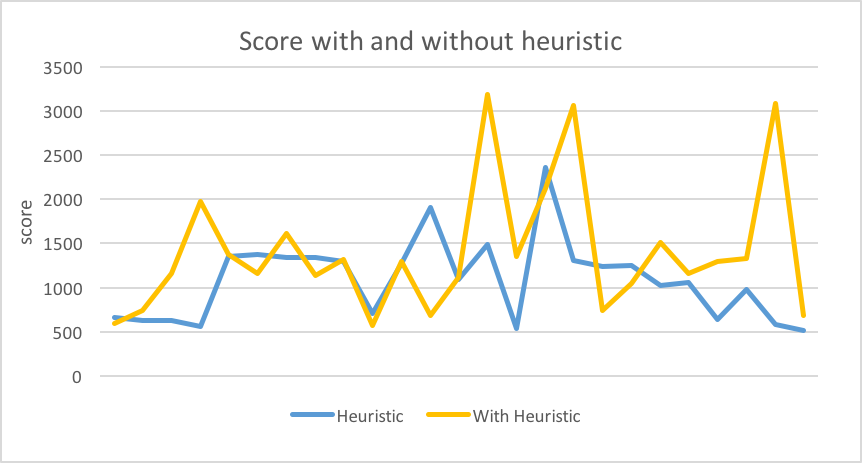
\includegraphics[width=4in]{images/hcomparison.png}}
\end{figure}

In order to confirm that our implementation was in fact following the algorithm as expected, we recorded the average score received by our AI at a number of different computational benchmarks in experiment, with the expectation that, if this AI indeed conducts Monte Carlo tree search, this would be a monotonic increase. This was indeed the case as you can see \textbf{Figure 3}, at a 1 iteration limit, the AI receives an average score of 987, just below the mean score of a random player, but as the number of iterations allowed increases, the AI steadily improves. In fact, in our tests, our AI was able to beat the random player consistently with as little as 4 iterations. This too, is consistent with UCT, as 4 iterations would allow the algorithm to sample all possible moves in order to inform its search. \\

Ultimately, with a 100 iteration limit---about a second per move on our computers---the AI earned an average score of 9015, significantly higher than the random strategy. In nearly all trials, the AI earned at least a 512 tile; in the majority of trails (71\%) it achieved the at least the 1024 tile; and in a small fraction (9\%) of trials, the AI earned a 2048 tile and hence beat the game.\\

Additionally, the AI was able to play reasonable well in several variations of \textit{generalized-2048}. Though the mean score varied between the scoring systems, the AI's intelligent behavior is indicated by the result that the average number of moves in the standard, sum and logsum scoring standards are all greater than the 109.1 average moves of the random player (161, 151.8 and 152.6, respectively).\\

Furthermore, we tested the standard UCT player without any domain-specific knowledge against one which incorporated the monotonicity heuristic into its tree policy. The result shown in \textbf{Figure 2} is that, with time held constant, the heuristic AI performed significantly better on average, with a mean score of 1412.16 as opposed to 1085.29 without the heuristics. We also note in Table 1 that the variance of scores with the heuristic decreases significantly, indicating that, in addition to increasing the average score, the incorporation of the heuristic also made the predictions of the AI more accurate, leading to more consistent final results. \\

\begin{figure}
\caption{Positive correlation between performance and number of iterations between}
\centerline{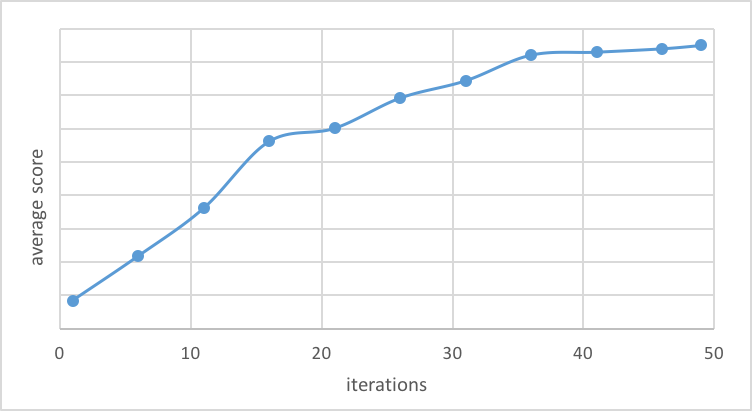
\includegraphics[width=3in]{images/scorevsiterations.png}}
\end{figure}


% Analysis, evaluation, and critique of the algorithm and your
% implementation. Include a description of the testing data you used and
% a discussion of examples that illustrate major features of your
% system. Testing is a critical part of system construction, and the
% scope of your testing will be an important component in our
% % evaluation. Discuss what you learned from the implementation.

\begin{table}
  \centering
  \begin{tabular}{lll}
    \toprule
    & Average Score & Variance\\
    \midrule
    Random & 1103 & 8.2 e4 \\
    UCT alone & 8457 &  5.6 e5\\
    UCT with heuristic & 9015 & 2.0 e5\\
    \bottomrule
  \end{tabular}
  \caption{UCT with heuristic performed consistently better than standard UCT}
\end{table}

\medskip

\section{Discussion}
Overall, the AI player significantly under-performed in comparison to the several published heuristic implementation, especially the highly-tuned ExpectiMax solution. Several weaknesses in our implementation likely contribute to this fact. Most significantly, perhaps, is that the implementation is relatively slow, constraining the amount of iterations it can conduct for its planning in a reasonable amount of time for each move. After all, MCTS is highly sensitive to computational power; the more computation is available to the algorithm, the more successful of a move it is likely to find. As the trend in \textbf{Figure 3} indicates, an increase in the amount of iterations allowed is expected to lead to an increase in performance. In future implementations we aim to reduce this weakness via optimizations such as parallelization of the rollout simulations and using a faster language, such as C++, with which we can utilize more efficient data structures. \\

Due to these shortcomings, our results do indicate that MCTS methods are not an optimal path for \textit{2048} AI solutions. One reason for this may be the relatively low branching factor of 4 in its game tree, especially when compared to a game such as Go, which has a branching factor of 250, making it a game ideal for MCTS. Perhaps, for this reason, ExpectiMax is the superior algorithm in this case, since a strict comparison of alternatives at each step is computationally feasible, and, given the simplicity of the game, building reasonable heuristics is achievable. Our hope that depth of the game tree might tip the scale in the favor of MCTS methods turned out to be unfounded, perhaps due to the effectiveness of the heuristics. Another possibility is to incorporate learning in our MCTS search as did Rolet et al.\cite{learning-mcts} and the AlphaGo solution \cite{nature_alpha_go}, so that our AI can dynamically improve.\\


% Summary of approach and results. Major takeaways? Things you could improve in future work?
\appendix
\section{System Description}
%  Appendix 1 � A clear description of how to use your system and how to generate the output you discussed in the write-up. \emph{The teaching staff must be able to run your system.}
All code is contained within the src/game/ subfolder. A number of settings and parameters can be tuned in the constants.py file. This includes practical settings such as display options and implementation settings such as the computational budget you'd like to set for each move. To run an experiment with the chosen settings, navigate to to the the src/game/ folder in the terminal and run the command:

\begin{center}
\textbf{python main.py -n \{number of trials\} -f \{outfile\}}\\
\end{center} 

The outfile will be left in the same folder in a csv file \texttt{outfile.csv} that contains score and highest tile data from the trials in the experiment.


\section{Group Makeup}
Ahmed Ahmed and Paul Lisker completed this project together.

\section{Code}
Our complete code can be found here: \url{https://github.com/plisker/GGP-2048}.

\bibliographystyle{plain} 
\bibliography{lisker_ahmed_ggp}

\end{document}
